\documentclass[11pt,a4paper]{article}
\usepackage{tikz}
\usetikzlibrary{arrows.meta,positioning}
\usepackage{tabularx}
\usepackage{amsmath,amssymb,amsthm}
\usepackage{geometry}
\geometry{margin=1in}
\usepackage{hyperref}
\usepackage{graphicx}
\usepackage{setspace}
\onehalfspacing

\title{\textbf{Paper F-03: Black Hole Thermodynamics:\\ A Constraint-Driven Flux Dynamics (CDFD) Perspective}}
\author{Steve Bico Mujjabi, MD\\
\small Independent Researcher\\
\small Founder, Vura Labs\\
\small Kampala, Uganda\\
\small ORCID: 0009-0001-0556-5516}
\date{August 2026}

\begin{document}
\maketitle

% BEGIN SHARED-METHODS POINTER
\noindent\textit{Shared Part IV notation and evidence boundaries are defined in \path{PART_IV_METHODS_AND_CLAIM_BOUNDARY.md}. This paper states only its local observables, comparison, and failure conditions.}
% END SHARED-METHODS POINTER


\begin{abstract}
This paper develops a falsifiable CDFD/AFL model of Black Hole Thermodynamics. It maps mass, energy, angular momentum, magnetic flux, and accretion to driving flux $\Phi$, horizon geometry, gravity, radiative efficiency, and disk transport to active constraint $C$, disk reconfiguration, jets, outflows, and environmental feedback to responsiveness $S$, and spin, charge, growth, magnetic topology, and accretion history to structural memory $M_s$. The target outcome is luminosity, growth, jet power, and thermodynamic accounting, tested against gravitational waves, spectra, timing, imaging, accretion estimates, and simulations. The paper treats universality as a shared model architecture rather than an assertion that unlike systems have the same material mechanism. It states the negative result that would make the mapping unnecessary and places the domain claim inside the cumulative CDFD programme and its reproducible runtime boundary.
\end{abstract}

\section{Introduction}

In standard relativistic frameworks, a black hole is a region of spacetime exhibiting such strong gravitational acceleration that nothing, including light, can escape. The boundary defining this region is the event horizon. Following the works of Bekenstein and Hawking, the event horizon is understood to possess an entropy proportional to its surface area, $S_{BH} = \frac{k_B A}{4 l_p^2}$, suggesting that all the information of the infalling volume is holographically encoded on the 2D boundary.

The CDFD paradigm posits that the universe is governed by the continuous interaction of flow ($\Phi$) and constraint ($C$) across adaptive surfaces. In this context, a black hole is not a singularity of broken physics; rather, it is the maximal boundary condition of the CDFD equations. It is the extreme limit where constraint $C$ approaches infinity for classical flow, forcing all throughput to undergo quantum phase transitions.

\section{The Event Horizon as an Active Surface}
In the CDFD framework, any boundary separating two topological regions evaluates to an active surface governed by the equation:
\begin{equation}
    \Psi_s = \left( \frac{\Phi}{C} \right) \cdot S \cdot M_s
\end{equation}

For an event horizon, the parameters map as follows:
\begin{itemize}
    \item \textbf{Flux ($\Phi$)}: The accretion of matter and information crossing the boundary (inward), and Hawking radiation (outward).
    \item \textbf{Constraint ($C$)}: The causal barrier generated by extreme spacetime curvature. For macroscopic inward flow, the boundary allows absolute transmission. For outward classical flow, $C \to \infty$.
    \item \textbf{Responsiveness ($S$)}: The geometric surface area of the horizon $A$, which defines the thermodynamic capacity to process and encode incoming flux.
    \item \textbf{Memory ($M_s$)}: The holographic encoding. Every bit of information that crosses the horizon is chronicled on the surface. Therefore, the event horizon possesses perfect, unbroken memory, $M_s \to 1.0$.
\end{itemize}

\subsection{Information Bottlenecks and The Bekenstein Bound}
As matter falls into the black hole, the inward flux $\Phi_{in}$ causes the mass, and thus the surface area $S$, to increase. This constitutes a dynamic adaptation. The horizon expands its surface responsiveness precisely to accommodate the increased memory load $M_s$. The Bekenstein bound is essentially the limit of information density allowed by the constraint $C$.

If the black hole attempts to absorb flux faster than the surface can expand and encode it, the system would theoretically experience a $\Psi_s > 1$ "over-flux" anomaly. However, the geometric rigidity of General Relativity ensures that $S$ expands in lockstep with mass, maintaining $\Psi_s \approx 1$.

\section{Hawking Radiation as Regime Stabilization}
If an isolated black hole ceases to accrete matter ($\Phi_{in} = 0$), the static nature of the system threatens to drop the adaptive ratio $\Psi_s \ll 1$. In biological systems (AFL), a drop in throughput leads to decay. In the cosmological vacuum, the event horizon undergoes analogous decay to shed its memory load and lower its constraint profile.

Hawking radiation ($\Phi_{out}$) emerges as the necessary quantum leakage required to satisfy the CDFD equation. To prevent $\Psi_s \to 0$, the vacuum surface generates an outward flux at the expense of its own structural memory (mass/area). As the horizon shrinks, the temperature increases, amplifying $\Phi_{out}$ until complete evaporation occurs.



\section{Measurement Layer}

% BEGIN PART IV MAJOR CROSS-DOMAIN UPGRADE
\section{Cross-Domain Model Upgrade: Mechanism, Scale, and Tests}

\subsection{Observable Translation}

The paper-specific translation begins with an observable chain rather than a
verbal analogy. For Black Hole Thermodynamics, the proposed drive is mass, energy, angular momentum, magnetic flux, and accretion.
The active limitation is horizon geometry, gravity, radiative efficiency, and disk transport. Responsiveness is carried by
disk reconfiguration, jets, outflows, and environmental feedback, while retained state is represented by
spin, charge, growth, magnetic topology, and accretion history. The outcome to explain is luminosity, growth, jet power, and thermodynamic accounting.

\begin{table}[htbp]
\centering
\small
\caption{Operational CDFD/AFL map for Paper F-03.}
\begin{tabularx}{\textwidth}{|l|X|X|}
\hline
\textbf{Term} & \textbf{Paper-specific observable meaning} & \textbf{Measurement question} \\
\hline
$\Phi$ & mass, energy, angular momentum, magnetic flux, and accretion & What rate, load, gradient, or demand enters the focal system? \\
\hline
$C$ & horizon geometry, gravity, radiative efficiency, and disk transport & Which measured bottleneck limits transfer, function, or recovery? \\
\hline
$S$ & disk reconfiguration, jets, outflows, and environmental feedback & Which process changes effective capacity or reroutes the load? \\
\hline
$M_s$ & spin, charge, growth, magnetic topology, and accretion history & Which retained state makes equal present loads produce different futures? \\
\hline
$Y$ & luminosity, growth, jet power, and thermodynamic accounting & Which outcome is predicted out of sample, with uncertainty? \\
\hline
\end{tabularx}
\end{table}

\begin{figure}[htbp]
\centering
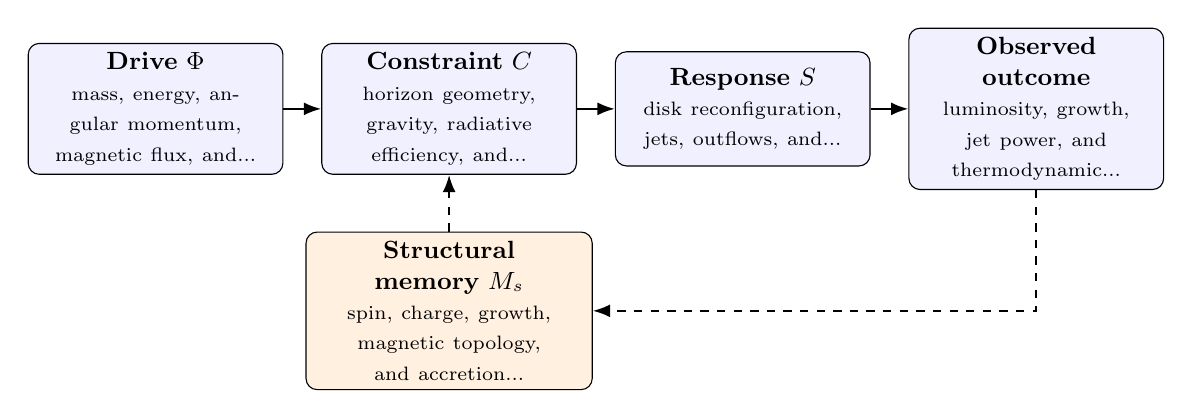
\begin{tikzpicture}[
    node distance=0.48cm,
    every node/.style={font=\small},
    box/.style={draw, rounded corners, align=center, minimum height=1.45cm, text width=3.0cm, fill=blue!6},
    memory/.style={draw, rounded corners, align=center, minimum height=1.25cm, text width=3.4cm, fill=orange!12},
    flow/.style={-{Latex[length=2.2mm]}, thick},
    feedback/.style={-{Latex[length=2.2mm]}, thick, dashed}
]
\node[box] (drive) {\textbf{Drive $\Phi$}\\\scriptsize mass, energy, angular momentum, magnetic flux, and...};
\node[box, right=of drive] (constraint) {\textbf{Constraint $C$}\\\scriptsize horizon geometry, gravity, radiative efficiency, and...};
\node[box, right=of constraint] (response) {\textbf{Response $S$}\\\scriptsize disk reconfiguration, jets, outflows, and...};
\node[box, right=of response] (outcome) {\textbf{Observed outcome}\\\scriptsize luminosity, growth, jet power, and thermodynamic...};
\node[memory, below=0.72cm of constraint] (memory) {\textbf{Structural memory $M_s$}\\\scriptsize spin, charge, growth, magnetic topology, and accretion...};
\draw[flow] (drive) -- (constraint);
\draw[flow] (constraint) -- (response);
\draw[flow] (response) -- (outcome);
\draw[feedback] (outcome.south) |- (memory.east);
\draw[feedback] (memory.north) -- (constraint.south);
\end{tikzpicture}
\caption{Paper F-03 observable CDFD/AFL architecture for Black Hole Thermodynamics. Solid arrows give the proposed forward chain; dashed arrows make history-dependent feedback explicit.}
\label{fig:f03-architecture}
\end{figure}

\subsection{Paper-Specific Causal Hypothesis}

For this paper, the hypothesized causal sequence is specific. A change in
mass, energy, angular momentum, magnetic flux, and accretion arrives faster than disk reconfiguration, jets, outflows, and environmental feedback can compensate.
This raises or redistributes horizon geometry, gravity, radiative efficiency, and disk transport. If the load persists,
the retained state encoded by spin, charge, growth, magnetic topology, and accretion history changes the next response, so a later event of equal
magnitude can produce a different trajectory in luminosity, growth, jet power, and thermodynamic accounting. The
scientific task is to estimate that sequence against the best ordinary model of
the domain, not merely to redescribe the outcome after it occurs.

\subsection{Cross-Scale Translation Without Mechanistic Erasure}

For the cosmic and subatomic systems family, the cross-domain translation must remain subordinate to conservation laws, relativity, quantum mechanics, and established astrophysical or plasma equations. CDFD is useful only if it compresses a regime transition or hysteresis question without pretending that biological adaptation and physical response are the same mechanism. \cite{Turing1952,Shannon1948,BakTangWiesenfeld1987}
The required scale declaration for this paper is microseconds to cosmic time; horizons to galactic environments. At short
scales, the key question is whether the incoming drive is transmitted,
buffered, or diverted. At intermediate scales, response changes effective
capacity and network exposure. At long scales, retained structure can alter the
state space itself. A result is genuinely cross-scale only when the aggregation
rule is stated and the same conclusion is not an artifact of averaging.

\subsection{Evidence Ladder and Discriminating Tests}

\begin{table}[htbp]
\centering
\small
\caption{Evidence ladder for Paper F-03. Each rung can fail independently.}
\begin{tabularx}{\textwidth}{|p{0.17\textwidth}|X|X|}
\hline
\textbf{Test} & \textbf{Design} & \textbf{Discriminating result} \\
\hline
Proxy audit & Measure gravitational waves, spectra, timing, imaging, accretion estimates, and simulations and preregister how each record maps to $\Phi$, $C$, $S$, $M_s$, and $Y$. & The mapping fails if proxies are non-identifiable, circular, or change meaning across cases. \\
\hline
Load ramp & Apply or observe an accretion-state transition at matched mass and environment while estimating the dominant constraint and response time. & A threshold claim requires a reproducible nonlinear change and uncertainty bounds, not a visually chosen breakpoint. \\
\hline
Recovery and memory & Match present load across units with different histories, then compare recovery paths. & The memory claim requires history-dependent divergence after current conditions are controlled. \\
\hline
Model comparison & Compare the baseline domain model with and without the CDFD/AFL state variables using held-out data. & The paper's stated falsifier is: CDFD introduces no distinguishable prediction beyond relativity and accretion physics. \\
\hline
\end{tabularx}
\end{table}

\subsection{Research Programme and Boundary Conditions}

The immediate research programme has four steps. First, construct a documented
dataset from gravitational waves, spectra, timing, imaging, accretion estimates, and simulations and retain raw units before normalization.
Second, fit a baseline domain model and report its calibration and out-of-sample
error. Third, add the smallest identifiable CDFD/AFL state extension and test
whether it improves prediction of luminosity, growth, jet power, and thermodynamic accounting. Fourth, repeat the
analysis across the declared scale range and publish negative cases as part of
the cross-domain translation audit.

% END PART IV MAJOR CROSS-DOMAIN UPGRADE

\section{Conclusion}
Black-hole thermodynamics and living systems can both be described with boundary, flux, and retained-state variables, but their mechanisms are not isomorphic. This paper limits the comparison to measurable accretion, horizon, spin, and radiation quantities and asks whether the CDFD translation adds anything beyond relativity and accretion physics.
\section*{Conflict of Interest} The author declares no conflict of interest.
\section*{Data Availability}
Part-specific runtime diagnostics are under each Part's \path{outputs/} directory.

Release-wide code: \path{Part_E_Synthesis/supplementary/}.

Generated summaries: \path{Part_E_Synthesis/outputs/}.

Figures: \path{Part_E_Synthesis/figures/}.


\section{Reference Layer}
\bibliographystyle{plain}
\bibliography{universal_afl_references}
\end{document}
